\chapter{Architektura i technologie}

Niniejszy rozdział został poświęcony ogólnemu opisowi architektury systemu oraz zastosowanych technologii. Dla poszczególnych wyborów zostały przedstawione przesłanki, którymi kierował się autor tej pracy. 

Istotnym czynnikiem mającym wpływ na wybór technologii oraz wzorców architektonicznych była chęć poszerzenia wiedzy autora niniejszej pracy w ich zakresie. Cechą wspólną wszystkich zastosowanych rozwiązań jest szeroki dostęp do materiałów w postaci dokumentacji oraz pozycji książkowych. 

\section{Architektura systemu}

Ze względu na potrzebę szerokiej dostępności platformy została ona zrealizowana jako system webowy w architekturze klient - serwer. Interfejsem użytkownika końcowego jest aplikacja kliencka typu SPA (ang. \textit{Single Page Application}) uruchamiana w przeglądarce internetowej. Aplikacja ta komunikuje się z API (ang. \textit{Application Programming Interface}) aplikacji serwerowej za pomocą zapytań protokołu HTTP (ang. \textit{Hypertext Transfer Protocol}).  Aplikacja serwerowa z kolei komunikuje się z bazą danych w celu odczytu oraz zapisu informacji za pomocą interfejsu JDBC (ang. \textit{Java DataBase Connectivity}). 

\begin{figure}[ht]
\centering
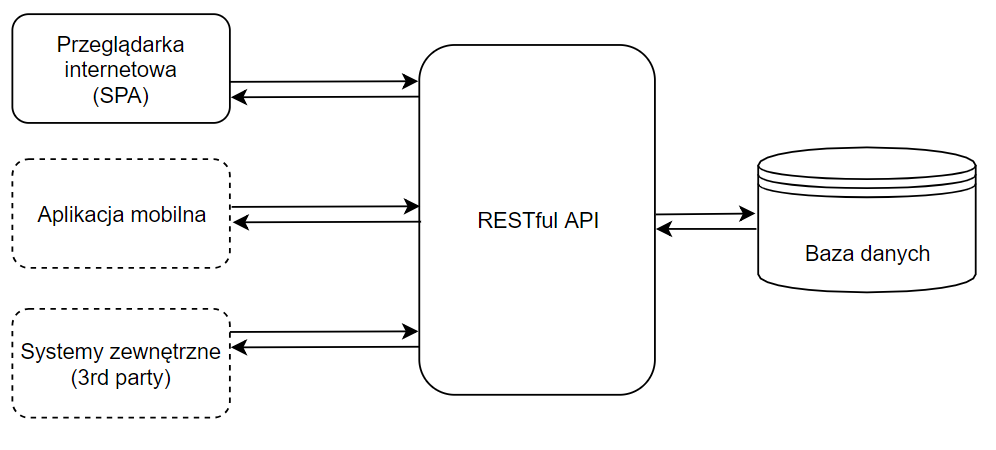
\includegraphics[width=0.8\linewidth]{05-architektura-i-technologie/rys/ogolna-architektura.PNG}
\caption{Diagram ogólnej architektury systemu}
\label{fig:diagram-og-architekt}
\end{figure}

Elementy otoczone linią kreskowaną na diagramie nie są przedmiotem tej pracy, jednak podkreślają uniwersalność API oraz wskazują możliwości rozwojowe oraz integracyjne systemu.

\subsection{RESTful API}
API wystawiane przez część serwerową zostało zaprojektowane w oparciu styl architektoniczny REST (ang. \textit{Representational State Transfer}), który zakłada komunikację klient-serwer z uwzględnieniem następujących zasad: 
\begin{itemize}
\item użycie podstawowych metody protokołu HTTP czyli - GET, PUT, POST oraz DELETE,
\item identyfikacja zasobów poprzez URL (ang. \textit{Uniform Resource Locator}),
\item komunikacja bezstanowa (brak sesji).
\end{itemize}

Użycie podstawowych metod protokołu HTTP pozytywnie wpływa na czytelność oraz intuicyjność API. Projektowanie z uwzględnieniem powyższych zasad pozwala również zminimalizować powiązania pomiędzy serwerem oraz klientem, API staje się uniwersalne. Otwiera to możliwości rozwoju systemu na inne platformy, np. utworzenie aplikacji klienckich dla systemów mobilnych \textit{Android} oraz \textit{iOs}. Możliwości rozwoju systemu zostały przedstawione za pomocą zakreskowanych bloków na rysunku~\ref{fig:diagram-og-architekt}.

\section{Stos technologiczny}

W poniższych sekcjach zostały przybliżone wybrane z zastosowanych technologii.  

\subsection{Java}

Aplikacja serwerowa została zaimplementowana w języku \textit{Java 1.8} \cite{java}. \textit{Java} jest bardzo często wybieranym językiem do budowy systemów internetowych, ze względu na duże wsparcie w postaci rozbudowanej biblioteki podstawowej, jak również dużą ilość darmowych narzędzi oraz bibliotek dostarczanych przez firmy trzecie. Język ten został wybrany również ze względu na doświadczenie akademickie oraz komercyjne autora niniejszej pracy, a także chęć dalszego rozwoju. 

Wersja 1.8 została wybrana ze względu na jej stabilność oraz dostarczone usprawnienia w postaci wyrażeń \textit{lambda}, przetwarzania strumieniowego oraz typu \textit{Optional}. Wymienione mechanizmy wpłynęły na zwiększenie wydajności procesu programowania oraz ogólnej jakości uzyskanego kodu.
 
\subsection{Spring Boot}

Podstawą dla rozwoju aplikacji serwerowej był szkielet \textit{Spring Boot} w wersji 2.0.3 \cite{springboot}. Główną zaletą budowy aplikacji sieciowej w oparciu o gotowy szkielet jest możliwość koncentracji na implementacji logiki biznesowej. Wiele mechanizmów związanych z obsługą zapytań, niezawodnością, bezpieczeństwem, dostępem do danych staje się odpowiedzialnością szkieletu aplikacji, a nie programisty. Programista ma możliwość konfiguracji oraz nadpisywania poszczególnych zachowań, jednak w wielu zastosowaniach okazuje się to być zbędne.


\subsection{JWT}

Technologia JWT (ang.\textit{Json Web Token}) została zastosowana jako sposób autoryzacji zapytań do API systemu. JWT jest technologią autoryzacji bezstanowej, przez co bardzo dobrze współgra z architekturą aplikacji REST-owych, dla których brak stanu jest jednym z głównych założeń.

\subsection{MySQL} 

Relacyjna baza danych została wybrana ze względu na dużą ilość powiązań między encjami w systemie. \textit{MySQL} od firmy \textit{Oracle} jest darmowym, bezpiecznym oraz wydajnym systemem zarządzania bazą danych.  Istotnym uzasadnieniem wyboru tej technologii jest również bardzo dobra integracja ze szkieletem \textit{Spring}.

\subsection{Angular}

Główną technologią wykorzystywaną po stronie front endu jest szkielet do tworzenia SPA (ang. \textit{Single Page Application}) rozwijany przez firmę \textit{Google} - \textit{Angular} (w wersji 6.1.0) \cite{angular}. Szkielet ten ułatwia budowę skalowalnych i szybkich aplikacji z bogatym interfejsem użytkownika. Dużą zaletą \textit{Angular-a} jest wsparcie dla programowania w języku \textit{TypeScript}, co usprawnia rozwój aplikacji poprzez kontrolę typów.

Dodatkowo w celu usprawnienia procesu rozwoju aplikacji została wykorzystana biblioteka ngrx (w wersji 6.1.0), wspomagająca zarządzanie stanem aplikacji. Wykorzystanie tej biblioteki znacznie ułatwiło analizę działania aplikacji oraz diagnozowanie błędów.


\subsubsection{AntDesign - NgZorro}

\textit{NgZorro} zostało użyte jako główna biblioteka dostarczająca szeroką gamę komponentów graficznych do aplikacji w technologii \textit{Angular} \cite{ngzorro}. Wybór padł na to rozwiązanie ze względu na duże wsparcie dla przeglądarek oraz bardzo dobrą dokumentację z przykładami. Użyte komponenty również cechują się atrakcyjnym wyglądem, który ma duży wpływ na odbiór systemu przez użytkownika.

\subsection{Heroku}

\textit{Heroku} zapewnia duże wsparcie dla systemów zbudowanych w oparciu o język Java. Rozwiązanie to zostało wybrane ze względu na darmowe plany użytkowania, dobrą dokumentacje, jak również doświadczenie autora pracy w zakresie wdrożeń na tę platformę. 

Wdrożenie na \textit{Heroku} aplikacji w technologiach \textit{Spring Boot} oraz \textit{Anuglar} nie stanowi żadnego problemu. Platforma dostarcza również dodatek w postaci bazy \textit{MySQL}. W przypadku darmowego planu pojemność bazy jest bardzo ograniczona, jednak wystarczająca w celach rozwojowych oraz weryfikacyjnych systemu.